% ----------------------------------------------------------- %
\chapter{Materials and Methods}
\label{sec:materials_methods}


In the previous chapter, it was possible to note that despite the important computational advancements in predicting CDGs, there are still several methodological challenges that require attention. One area that remains underexplored is the use of graph-based learning algorithms, such as graph neural networks. However, given the increasing success of GNNs in bioinformatics applications as reviewed by \citet{zhang2021graph}, exploring the potential of these algorithms for predicting CDGs is a promising research direction.

Thus, the primary focus of this work is to investigate the potential of GNNs for predicting CDGs and develop a model that can efficiently leverage information contained in PPI networks and multi-omics data to learn patterns related to CDGs. Our approach is motivated by findings from previous research highlighting that a node context within a biological network provides valuable information for predicting cancer drivers \cite{Gumpinger2020}. 

To develop a graph-based predictive model for CDG discovery, we conducted a comprehensive analysis of several important aspects related to model development, including the choice of PPI networks and omics data employed as node features, the use of distinct GNN algorithms, and the strategies adopted for handling class imbalance. Furthermore, we proposed ensemble-based approaches to improve the predictive performance of individual models.  A summary of our methodology is provided in Figure~\ref{fig:metodologia}. 

This chapter details the materials and methods utilized in this work, providing an overview of each methodological step involved in both the comprehensive experimental investigation of learning algorithms and data representation (reported in Chapter~\ref{sec:results:comparative_evaluation}) and the development of a GNN model for CDGs prediction (reported in Chapter~\ref{sec:gcn_model}).


\begin{figure*}[!th]
    \centering
    \caption{Methodology employed in the current work for model development.}
    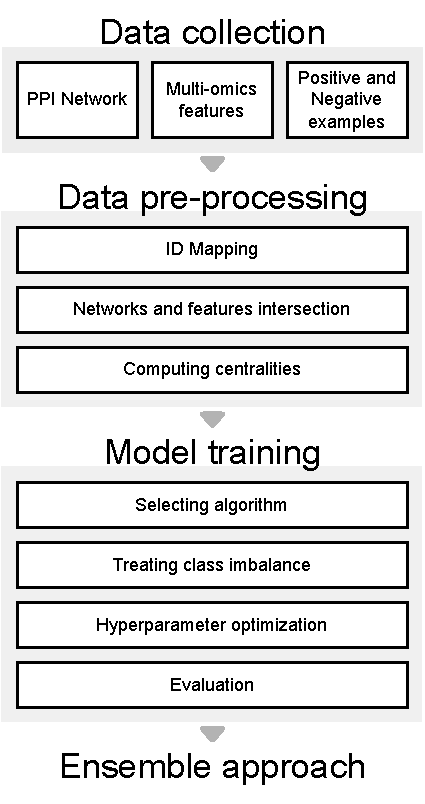
\includegraphics[width=0.5\textwidth]{images/testes/metodologia2.pdf}
    \legend{Source: Prepared by the author}
    \label{fig:metodologia}
\end{figure*}



\section{Data collection}

All the data employed in this work derive from publicly available sources. The following sections detail our data collection process to obtain protein-protein interaction networks (\ie our graphs used as the basis for learning),  omics data (\ie our node features), and gene annotations regarding their role in causing cancer (\ie our node labels). Figure~\ref{fig:fig_omics} illustrates how these different types of data are integrated, summarizing the multi-omics data collected.


\begin{figure*}[!ht]
    \centering
    \caption{Multi-omics Data Collection}
    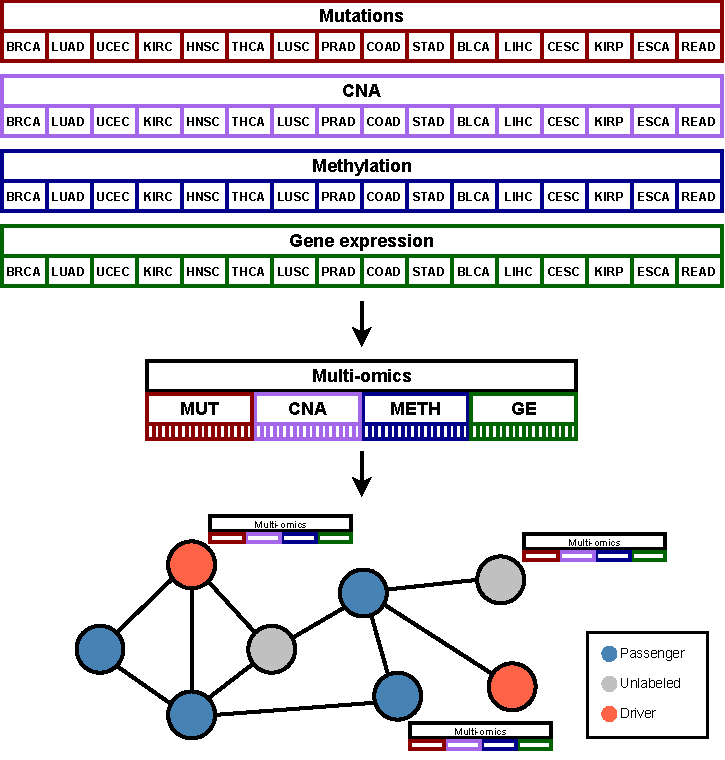
\includegraphics[width=0.9\textwidth]{images/revisadas/omics_features.pdf}
    \legend{Source: Prepared by the author}
    \label{fig:fig_omics}
\end{figure*}

\subsection{Protein-protein interaction networks}
\label{sec:materials_methods:ppinets}

As explained in Section~\ref{sec:background_ppi}, PPI networks depict the physical or functional relationship between proteins (\ie the nodes of the networks). Several databases provide organized and structured information about PPI networks. In this work, we adopted a reference database for the retrieval of molecular networks in human diseases research, named the Network Data Exchange (NDEx) \cite{pratt2015ndex, pillich2017ndex, pratt2017ndex}. The NDEx Project\footnote{Network Data Exchange (NDEx): \url{https://www.ndexbio.org/}} is a web-based resource that allows for the storage, sharing, manipulation, and publication of biological network models in human disease research \cite{pratt2015ndex, pillich2017ndex, pratt2017ndex}.


From the NDEx repository, we selected six pre-processed PPI networks that were deposited by \citet{huang2018systematic} in a study that performed a systematic evaluation of molecular networks regarding their ability to recover gene sets that characterize human diseases. Specifically, we downloaded the following networks: Human Protein Reference Database (HPRD), MultiNet, IRefIndex (IREF), Consensus Path DB (CPDB), Parsimonious Composite Network (PCNET), and Search Tool for Recurring Instances of Neighboring Genes (STRING). These networks were chosen because they vary in size, comprising from 30,000 (HPRD) to 5 million (STRING) molecular interactions. Moreover, PCNET showed the highest performance in retrieving the disease-associated gene sets among a total of 21 networks evaluated in the original work \cite{huang2018systematic}.


PPI networks are typically represented as undirected and unweighted graphs (similar to the citation networks used in original GCN applications \cite{kipf2016semi}). Although the NDEx repository provides edge weights for some PPI networks, which represent the total weight of evidence for an interaction between two proteins, we discarded this information for all PPI networks used in this study. The PPI networks had already undergone a normalization process to enable comparison among them. In the original study \cite{huang2018systematic}, only interactions among protein-coding genes were kept, and all nodes (proteins) were mapped to their corresponding Gene Symbols provided by HUGO Gene Nomenclature Committee (HGNC). However, because this data was compiled in 2018, PPI data underwent another normalization process for nomenclature in our study, which will be later explained in Section \ref{sec:materials_methods:idmapping}. 


Finally, we defined a large consensus PPI network by merging the six selected PPI networks into a single network and removing duplicated edges. This PPI network is the most comprehensive among all collected interaction datasets and it aims to evaluate how the algorithms perform for larger and denser networks.
We call this merged network the UNION PPI network, which is composed of more than 7.5 million interactions. Details about the original number of nodes and edges in each PPI network are provided in Table~\ref{tab:ppi_networks_colected}.

\begin{table}[!h]
\centering
\caption{Number of nodes and edges in PPI networks \label{tab:ppi_networks_colected}}
\resizebox{\textwidth}{!}{
\begin{tabular}{cccccccc}
\hline
 & HPRD & MULTINET & IREF & CPDB & PCNET & STRING & UNION \\ \hline
Edges & 36,867 & 109,595 & 133,548 & 1,648,426 & 2,724,724 & 5,135,768 & 7,515,970 \\
Nodes & 9,453 & 14,445 & 14,667 & 16,301 & 19,781 & 18,266 & 21,968 \\ \hline
\end{tabular}}
%}
\end{table}



\subsection{Omics data}
\label{sec:materials_methods:omics}

Integrating different types of omics data in the discovery of CDGs is a common approach, as discussed in Chapter~\ref{sec:related_works}, since each type of omics carries a distinct, partial view about the molecular changes associated with cancer. In this work, we followed this trend and collected four types of omics data interrogating SNVs, CNAs, DNA methylation, and gene expression in a large scale (see Section~\ref{sec:background:bio_data} for theoretical background). The datasets were originally produced by the TCGA project and comprise over 8,000 samples from 16 different cancer types. We downloaded a version of the data that was pre-processed by a previous study \cite{schulte2021integration} to create informative features from this genome-wide molecular data. The authors defined computational features as relative values comparing a quantity of a biological feature in tumor sample compared to a matched normal sample from the same cancer type. Due to this definition, the analysis was limited to those cancer types with data available for both cancer and normal samples, as listed in Table~\ref{tab:cancer_types}.




\begin{table}[!bh]
\centering
\caption{List of cancer types included in the omics data analyzed. \label{tab:cancer_types}}
\begin{tabular}{ll}
\hline
\multicolumn{1}{c}{Abbreviation} & \multicolumn{1}{c}{Cancer Type Description} \\ \hline
BRCA & Breast invasive carcinoma \\
LUAD & Lung adenocarcinoma \\
UCEC & Uterine Corpus Endometrial carcinoma \\
KIRC & Kidney renal clear cell carcinoma \\
HNSC & Head and Neck squamous cell carcinoma \\
THCA & Thyroid carcinoma \\
LUSC & Lung squamous cell carcinoma \\
PRAD & Prostate adenocarcinoma \\
COAD & Colon adenocarcinoma \\
STAD & Stomach adenocarcinoma \\
BLCA & Bladder Urothelial Carcinoma \\
LIHC & Liver hepatocellular carcinoma \\
CESC & Cervical squamous cell carcinoma and endocervical adenocarcinoma \\
KIRP & Kidney renal papillary cell carcinoma \\
ESCA & Esophageal carcinoma \\
READ & Rectum adenocarcinoma \\ \hline
\end{tabular}
\end{table}




In what follows, we briefly mention the pre-processing steps conducted by \citet{schulte2021integration}; more details can be obtained in the original work.
 

\begin{itemize}
    \item \textbf{SNVs:} the somatic mutation provided in Mutation Annotation Format (MAF) was subject to statistical analysis for variants calling following the pipeline from HotNet2 \cite{leiserson2015pan}. Silent mutations were removed from data to concentrate on SNVs that have an effect on the mRNA or protein. A normalized mutation rate (\ie SNV frequency) was computed for each gene in each cancer type, by dividing the number of non-silent SNVs in that gene its by exonic length. 
    \item \textbf{CNAs:} copy number alterations detected through DNA sequencing were analyzed with GISTIC2 \cite{gistic2} to identify the exact amplified or deleted target genes. Ultra-mutated samples from TCGA were removed. The copy number rate of a certain gene in a TCGA cohort was defined as the number of times a gene was amplified or deleted in that specific cohort.
    \item \textbf{DNA methylation}: the DNA methylation status was analyzed for the promoter region of genes, defined as the region of $\pm$1000 base pairs around the Transcription Start Site (TSS) of that gene. Probes annotation was carried out with Gencode. Within the promoter region, the average $beta$ value (\ie DNA methylation signal) across all probes was used to determine the DNA methylation status of the gene. The $beta$ value ranges between 0 and 1 and describes the portion of cells that are methylated in the sample. For each gene, the average differential DNA methylation was computed by averaging the difference between the $beta$ values for a cancer sample and its matched normal sample across all samples in a given TCGA cohort.
    \item \textbf{Gene expression}: authors used the data from \citet{wang2018unifying}, in which gene expression levels for TCGA cancer samples were combined with gene expression data for normal samples of the same tissue produced by the  Genotype-Tissue Expression (GTEx) consortium in a controlled protocol to ensure similar distributions among cancer and normal samples. The differential expression for a gene in a given cancer sample was calculated as a log2-fold change between the expression values in the cancer versus a matched normal sample. Finally, for each gene, an average differential expression was computed across all samples from the same cancer type.
\end{itemize}



After individual pre-processing, each type of omics data results in a feature matrix in the form of $N \times 16$, in which $N$ denotes the number of genes and 16 refers to the number of TCGA cancer cohorts analyzed (as illustrated in Figure \ref{fig:fig_omics}). Thus, for each gene, we obtained 16 features corresponding to its molecular profile in terms of SNVs, CNAs, differential DNA methylation or differential gene expression across 16 types of cancer. Each feature matrix was passed through min-max normalization to ensure similarity among the scale of the different types of omics data in joint analyses. Besides the individual features matrices, we also generated a multi-omics feature matrix by simply concatenating the four individual feature matrices for the individual omics levels, generating a $22,193 \times (4 * 16)$ matrix.


\subsection{Positive and negative examples of CDGs}
\label{sec:materials_methods:cdglabels}

To create a reliable list of labeled genes, we examined catalogs of cancer-causing genes available in previous studies or public databases. We defined two main sets of genes: the positively labeled genes, which are \textit{driver genes}, and the negatively labeled genes, which are \textit{non-cancer genes} or \textit{passenger genes}. However, many genes do not fall into either of these categories because they have some evidence of involvement in oncogenesis but lack definitive annotation to be considered as true drivers, or because they have been associated with other diseases, increasing their chance to be cancer-related genes. These genes are referred in our work as the \textit{unlabeled} set, but we note that they may still represent potential candidate driver genes. The data collection process for these gene sets is elaborated in the following paragraphs.

We obtained six lists of genes to be processed as necessary for creating node labels for our networks: (i) driver and candidate drivers from the Network of Cancer Genes (NCG) version 7.0 \cite{repana2019network}; (ii) Tier 1 and Tier 2 lists from the Cancer Gene Census (CGC) available in COSMIC v95 \cite{cosmic}; (iii) the OncoKB Cancer Gene List (version of July 1st, 20222) \cite{chakravarty2017oncokb}; (iv) a compilation of cancer genes organized by Bushman Lab\footnote{Available at \url{http://www.bushmanlab.org/links/genelists}} (v5, from June 2021); (v) genes related to cancer pathways in the Consensus Path DB (CPDB) (Release 35, updated on 05/06/2021) \cite{consensuspathdb}; and (vi) disease-associated genes registered in the Online Mendelian Inheritance in Man (OMIM) \cite{hamosh2000online}. All gene lists were downloaded at January 14th, 2022.

For positive examples of CDGs, we collected a list of canonical cancer drivers from NCG 7.0 (591 genes), the Tier 1 list from CGC (578 genes) that contains genes with cancer gene mutation patterns and documented activity relevant to cancer, and a list of TSGs and OGs from OncoKb (500 genes). Combining the three lists and removing the duplicated genes, we arrive at 907 positive genes.

Next, we compiled a list of disease candidate genes, which are those gene implicated in other diseases or that have indications of an oncogenic role (\eg through computational prediction) but the body of scientific evidence supporting their role is still emerging, thus, they lack strong experimental evidence to be labeled as positive examples of cancer drivers. We collected the list of candidate cancer drivers from NCG 7.0 (3177 genes), the Tier 2 list from CGC (151 genes), the cancer-related gene list provided by the Bushman Lab (2580 genes), and the cancer gene list from OncoKB excluding annotated TSGs and OGs (500 genes). We also obtained a list of genes annotated in cancer pathways according to CPDB (4333 genes) and a list of genes previously associated with other human diseases according to OMIM (2143 genes). Again, as redundancy may exist when integrating the lists obtained from different data sources, many duplicates were found and removed. Moreover, genes that were classified as drivers in any of the sources previously mentioned were removed from the list. We obtained a total of 5777 unique disease candidate genes that were grouped as the \textit{unlabeled} gene set. These genes were treated as unlabeled nodes in our computational prediction approach, since the uncertainty about their role in oncogenesis prevents us from considering true cancer drivers, but it is risky to label them as passenger ones due to existing evidence of association with cancer or other diseases. 

Given that the definition of robust negative examples of CDGs is more challenging, as mentioned in Chapter~\ref{sec:related_works}, we followed a similar strategy applied in previous works and filtered the list of genes available in the collected PPI networks and omics data to remove all genes with previously reported association with cancer or other diseases (including strong and weak evidences). Thus, we considered as negative examples (\textit{non-cancer genes}), all the genes in our data that were not included in any of the following lists: the compiled list of positive examples of CDGs, the candidate cancer genes list, the cancer pathways gene list from CPDB, and the disease-related genes list from OMIM. In summary, negative examples of CDGs are those that do not appear in the defined  \textit{driver} gene set or in the defined \textit{unlabeled} gene set.

With the complete list of positive and negative examples of CDGs, it is possible to cross this information with the genes present in each PPI network to define node labels distribution per network. This process and other pre-processing steps will be detailed in the next section. However, the final class label distribution per PPI network is shown in Figure~\ref{fig:chart_labels}. We can observe the high class imbalance in the dataset, with the driver genes representing the minority class.


\begin{figure*}[!th]
    \centering
      \caption{Final distribution of class labels per PPI network.}
    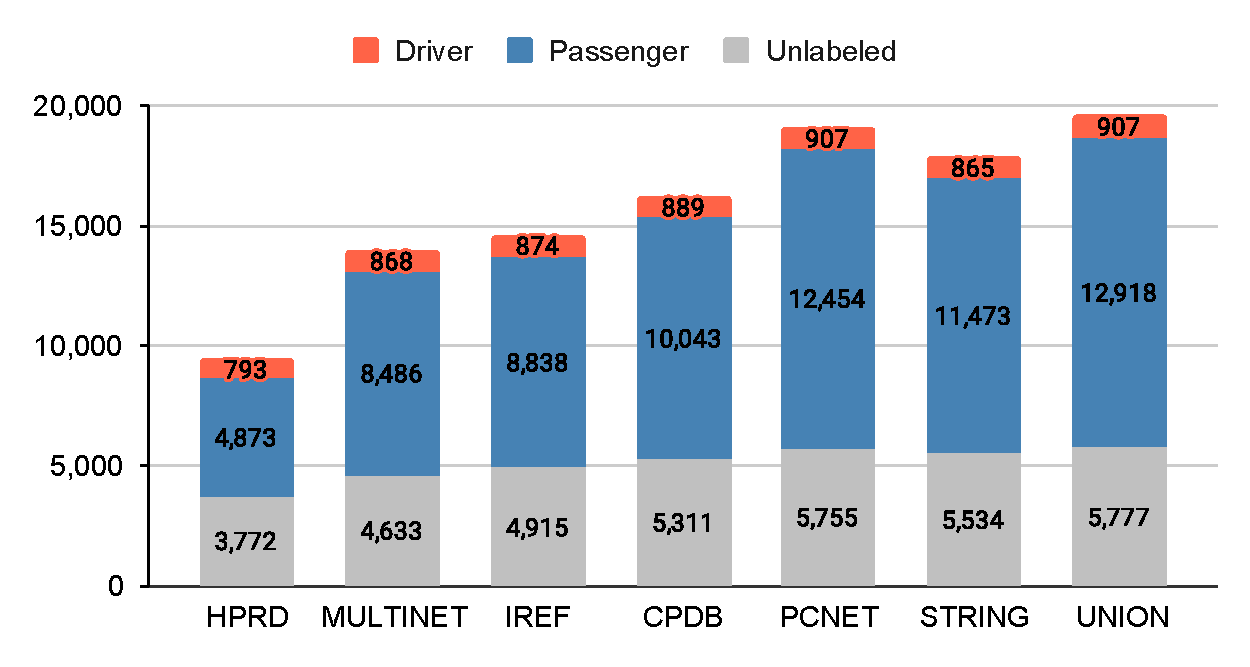
\includegraphics[width=\textwidth]{images/ilustracoes/chart_labels.pdf}
    \legend{Source: Prepared by the author}
    \label{fig:chart_labels}
\end{figure*}


\section{Data pre-processing}
\label{sec:materials_methods:datapreproc}

All collected data were subject to further pre-processing to allow creating a consistent training data for the learning algorithms explored in this work. In this section, we describe the steps involved in data pre-processing, which comprise (i) mapping gene IDs, (ii) intersecting genes among PPI networks and omics data, and (iii) extracting node centralities from PPI networks. 


\subsection{Gene ID mapping}
\label{sec:materials_methods:idmapping}

To carry out the experiments for model training with ML or DL, the nodes IDs need to be standardized across the various data sources that are collected in this work. As mentioned earlier, the genes of the PPI networks are standardized in Gene Symbols provided by HUGO Gene Nomenclature Committee (HGNC), however the networks were last updated in 2018. The HGNC is a committee within the Human Genome Organization (HUGO), which frequently update its databases and has a curated online repository of HGNC-approved gene nomenclature. 

To ensure that we have the most up-to-date gene IDs, we used the HGNC Multi-symbol checker. This tool allows the user to upload a list of gene symbols in a search field to verify if they are HGNC approved symbols. The results include a ``match type'' column that shows how each queried symbol matches the returned HGNC symbol -- if either with approved HGNC symbols, alias symbols, updated symbols, or if the queried gene symbol has been withdrawn from database or if it did not return any match. 
Based on these results, we created a dictionary with the list of query genes and their corresponding approved symbols. We conducted the query on November 26th, 2021, and downloaded a complete dictionary of gene ID mappings that was used throughout all experiments. 

Table \ref{tab:translate_table} shows the original number of nodes in each of the seven PPI networks used and the resulting number of nodes after gene ID mapping. It is important to note that some nodes, and their connected edges, may have been removed from the network if their original ID could not be mapped to the updated HGNC gene symbols. This may lead to a reduction in the number of edges as well.



\begin{table}[!ht]
\centering
\caption{Original and modified number of nodes and edges in PPI networks as a result of data pre-processing steps. \label{tab:translate_table}}
\begin{tabular}{lcccccc}
\hline
\multicolumn{1}{c}{PPI Networks} & \multicolumn{2}{c}{Original}                & \multicolumn{2}{c}{Gene ID mapping}     & \multicolumn{2}{c}{Omics intersection}   \\ \hline
                                 & Edges                & Nodes                & Edges                & Nodes                & Edges                & Nodes                \\ \cline{2-7} 
                                 & \multicolumn{1}{l}{} & \multicolumn{1}{l}{} & \multicolumn{1}{l}{} & \multicolumn{1}{l}{} & \multicolumn{1}{l}{} & \multicolumn{1}{l}{} \\
HPRD                             & 36,867               & 9,453                & 36,852               & 9,444                & 36,844               & 9,438                \\
MULTINET                         & 109,595              & 14,445               & 108,568              & 13,987               & 108,568              & 13,987               \\
IREF                             & 133,548              & 14,667               & 133,100              & 14,632               & 133,095              & 14,627               \\
CPDB                             & 1,648,426            & 16,301               & 1,641,909            & 16,251               & 1,641,849            & 16,243               \\
PCNET                            & 2,724,724            & 19,781               & 2,712,881            & 19,116               & 2,712,881            & 19,116               \\
STRING                           & 5,135,768            & 18,266               & 5,028,709            & 18,044               & 5,002,412            & 17,872               \\
                                 & \multicolumn{1}{l}{} & \multicolumn{1}{l}{} & \multicolumn{1}{l}{} & \multicolumn{1}{l}{} & \multicolumn{1}{l}{} & \multicolumn{1}{l}{} \\
UNION                            & 7,515,970            & 21,968               & 7,391,452            & 19,792               & 7,365,082            & 19,602               \\ \hline
\end{tabular}
\end{table}


\subsection{Intersection of PPI networks and omics data}

In the proposed approach, a prediction model is built from the joint use of PPI networks and omics data through GNNs. The PPI network provide the fundamental graph structure for the graph-based learning, whereas the omics data provide node features that enrich node embeddings generated for the classification task. Thus, it is imperative to ensure a correspondence among genes in the PPI networks and genes present in the multi-omics dataset. For each PPI network, we compared the genes in the network and the genes in the muli-omics data to keep in the PPI network only genes that are in the intersection among both datasets. After this step, the number of nodes and edges were updated again, as shown in Table \ref{tab:translate_table}. This step allowed all nodes from all PPI networks to have their own set of features.




\subsection{Extraction of node centralities}


In Section \ref{cap:basis_graph_centralities}, we provided definitions of four measures of node centralities: degree, betweenness, closeness, and clustering coefficient. In the present section, we provide a brief overview of the extraction and normalization procedures used to obtain these measures. We employed a network analysis package, called \textit{igraph} \cite{igraphpackage}, which is an open-source tool that can be implemented using various programming languages, including Python, R, Mathematica, and C/C++. The igraph provides a versatile network analysis that enables mining information from graphs, ranging from simple operations such as adding and removing nodes to more complex theoretical constructions such as community detection. The Python interface of igraph (version 0.9.8) is utilized in this work to compute the four node-level properties, as detailed below:
\begin{itemize}
   
    \item \textbf{Degree}: accepts either a singular node ID or a list of node IDs as an input parameter and returns the number of edges incident on a node of the graph. The output is a single integer or a list, based on the input parameter. Degree values were normalized by the min-max method to keep it contained in an interval from 0 to 1, similar to the range of values for the omics features.

    \item \textbf{Betweenness}: assigns higher betweenness centrality scores for nodes that appear more frequently along the shortest paths computed. The score returned by the function is not standardized, so the same min-max normalization is also used.

    \item \textbf{Closeness}: when assessing how many steps is required to reach every other node from a given node, a normalized value is obtained by the inverse average distance to all reachable nodes.

    \item \textbf{Clustering coefficient}: the function returns a score value between 0 and 1, that means the probability that the adjacent nodes of a given node $i$ are connected. Thus, it was not necessary to apply a normalization. However, when a node has a degree lower than two, there is no transitivity, so a parameter was defined to consider these cases as zero (by default they are defined as NaN).
\end{itemize}

The analysis of centrality values adds four features to each node in the PPI networks. One of the goals of our experiments is to evaluate the effect of using centrality measures as features in GNNs, as will be later discussed in Chapter~\ref{sec:results:comparative_evaluation}. We emphasize that the centrality measures for a given gene vary among PPI networks because they are highly dependent on the graph structure. Unlike omics-based features, which remain the same for a given gene across PPI networks, the centralities-based features differ among PPI networks.


\section{Model training and evaluation}

After data collection, two classes of algorithms were applied for model development: graph neural network algorithms, which are the focus of our work, and traditional machine learning algorithms, which served as baselines in our experimental comparison. While graph neural networks were applied following a semi-supervised learning paradigm, traditional ML algorithms were trained in a pure supervised learning approach. This section aims to clarify the technical details underlying the application of the learning algorithms to the collected data.




\subsection{Graph-based learning algorithms}
\label{sec:materials_methods:gnns}

One of the goals of our study is to conduct a comparison among graph-based learning algorithms. To achieve this, we utilized a library called StellarGraph \cite{StellarGraph}, which offers implementations for state-of-the-art GNNs. This Python library is built on TensorFlow 2 and Keras, as well as Pandas and NumPy. We selected StellarGraph for its ease of use, modularity, extensibility, and range of algorithms that solve many ML tasks on graphs, including node-level predictions, which enables a fairer comparison among algorithms using the same data representation format and library.

Graph-based model training was conducted primarily with StellarGraph, but also employing TensorFlow, Keras, Pandas, and scikit-learn for auxiliar functions.  Three GNN algorithms were selected for evaluation: Graph Convolutional Networks (GCN), Graph Attention Networks (GAT), and GraphSAGE (see Section~\ref{sec:deep_and_gnns} for technical details). Since the algorithms were selected for a categorical prediction task, the categorical cross-entropy loss function is used as the standard loss function. While some of our experiments were based on default hyperparameters for the applied algorithms (see Chapter~\ref{sec:results:comparative_evaluation} for details), other experiments addressed hyperparameters optimization in an extensive evaluation of selected methods (see Chapter~\ref{sec:gcn_model} for details). Section~\ref{sec:methods:hyperparameters} will elaborate more on the optimization of hyperparameters.

When employing GNN algorithms, the task of predicting CDGs is modeled as a semi-supervised node classification task. Semi-supervised learning on graphs leverages the propagation of information in a per-layer fashion to obtain more advanced node representations, thereby avoiding the need for labeled data for all nodes while making the best use of available prior knowledge. In our domain, there are positively and negatively labeled genes, as well as a large set of unlabeled genes due to the lack of definitive evidence regarding their role in oncogenesis. However, by propagating feature information among neighboring nodes in a layer-wise manner, GNNs can still enable the model to learn patterns that can help discriminate CDGs.
After training, the model can be used to predict the class of the unlabeled nodes. This setup is particularly well-suited for discovering associations between entities in biological networks, such as cancer driver genes, given the limited knowledge about biological and molecular mechanisms underlying diseases.



\subsection{Hyperparameters in GNNs: definitions and optimization}
\label{sec:methods:hyperparameters}

The success of ML and DL algorithms, including GNNs, is partly attributed to the configuration of their hyperparameters, which enable them to achieve superior results on a given dataset \cite{yuan2021systematic}. Therefore, it is crucial to comprehend the hyperparameters involved in the chosen algorithms and conduct hyperparameter optimization when feasible. Despite the high similarity among the GNN algorithms applied in this work (Section~\ref{sec:materials_methods:gnns}) in term of their propagation module, each algorithm has particular hyperparameters on their own that are, in general, introduced as a way to help the algorithm to stand out from previous approaches. Table \ref{tab:hyperparameters_gnns} presents a brief description for hyperparameters involved in GNNs training.


\begin{table}[!ht]
\centering
\caption{Hyperparameters of the selected GNN algorithms \label{tab:hyperparameters_gnns}}
\begin{tabularx}{\textwidth}{lX}
\hline
Hyperparameter & Description \\ \hline
Layer sizes & The number of hidden convolutional layers of the GNN used for training and the feature dimensions for each hidden layer.\\
 &  \\
Activation function & The non-linear transformation function that is applied to the input signal and outputs a value that is passed on to the next layer. \\
 &  \\
Dropout rate & The percentage of units in the hidden layers that are randomly dropped during training.\\
 &  \\
Learning rate & The step size for a model's weight updates to reach the minimum loss function.\\
 &  \\
Number of epochs & The length of the training or, in other words, the number of times the training data will pass through the neural network.\\
 &  \\
Loss function & The evaluation function to estimate how well the algorithm can model the input data, measuring the difference between the predicted output and the actual output. \\
 &  \\
Attention heads & The number of operations of the layer that are independently replicated K times, used for regularization process to avoid fitting.  \\
 &  \\
Attention dropout & The dropout rate applied to attention coefficients. \\
 &  \\
Batch size & The number of random samples that will be propagated through the network. \\
 &  \\
Number of samples & Number of neighboring nodes to sample at each level of the model \\ \hline
\end{tabularx}
\end{table}

However, the high number of hyperparameters in GNN algorithms is a primary challenge in developing effective predictive models, as several hyperparameters can significantly impact model performance. Furthermore, hyperparameters optimization is often computationally expensive, and there is no guarantee that the chosen configuration is the optimal choice without experimental comparison. However, it is possible to obtain suitable hyperparameters value guidelines based on prior research.
 
For instance, \citet{kipf2016semi} reported that two to three convolutional layers are sufficient for learning patterns with GCNs, such that we start our experiments with only two layers. As for the number of units per layer, it depends on the specific model, but we decided to initially employ 64 units. The optimal dropout rate for improving model performance can range from 0 to 1, with a 10\% dropout already able to enhance the performance. Dropout is implemented in GNNs by randomly removing edges from the graph during training. Thus, our experiments started with a dropout rate of 0.1. Meanwhile, the learning rate usually falls within the range of 0.1 to 0.0001, according to \citet{koutsoukas2017deep}. We adopted, initially, a learning rate of 0.001 with ADAM optimizer. Additionally, the number of epochs should be chosen based on the local computing capacity. Our exploratory experiments used 300 epochs for GNN model training.

Activation functions are used in all GNN components to incorporate the feature-topology coupling into the network. The activation function ReLU has been frequently used due to its superior performance in many prediction tasks \cite{goodfellow2016deep}. For our classification task, the recommended loss function by StellarGraph is categorical cross-entropy. Finally, batch size is the only hyperparameter common to all algorithms that receives different recommendations for distinct algorithms according to StellarGraph default values. GCN and GAT are full-batch models, which means the batch size is one, while GraphSAGE trains the model with a batch size of 50.

The hyperparameters discussed so far are shared among the three selected GNN algorithms. Nonetheless, some algorithms introduce other hyperparameters specific to their functioning. The GAT algorithm has two hyperparameters of its own, the attention heads and attention dropout (as described in Table \ref{tab:hyperparameters_gnns}), which we initially configured with the default values recommended by the library: 8 and 0.01, respectively. GraphSAGE includes a hyperparameter related to the number of nodes to sample, for which we also used the standard setup of 10 sampled nodes in the first layer and 5 sampled nodes in the second layer for a two-layer network.


In our study, we performed two rounds of experiments to evaluate the performance of GNN algorithms for CDGs prediction based on PPI networks. In the first round, we used the default hyperparameter values, as outlined in the previous paragraphs, while in the second round, we fine-tuned a GNN model using a hyperparameter optimization process based on a grid search and $k$-fold cross-validation. The specific hyperparameter grid used is described in detail in Chapter~\ref{sec:gcn_model}. However, we note that due to the computational complexity of the PPI networks, a large number of hyperparameter combinations can result in long execution times, demanding an adaptation to the methodology of training and evaluating models. To address this, we adopted a strategy where we first ran hyperparameter optimization for the three smallest PPI networks with less than 140,000 edges (HPRD, MULTINET, and IREF). Based on an analysis of these results, we simplified the hyperparameters grid and used a reduced number of combinations for the three largest PPI networks. Further details on this analysis can be found in Chapter~\ref{sec:gcn_model}.








\subsection{Traditional machine learning algorithms}

Four traditional ML algorithms were chosen as baseline methods in our experiments, namely Support Vector Machines (SVM), Random Forests (RF), Gradient Boosting Trees (GBT), and Artificial Neural Networks (ANN). A theoretical background for these algorithms was provided in Section~\ref{sec:comp_concepts:tradml}. For these methods, the prediction of CDGs was modeled as a conventional supervised classification task, in which labeled positive and negative examples are used to learn the data patterns and fit a predictive model that can be latter applied to classifiy unseen, unlabeled data.


The traditional ML algorithms were applied in our pipeline for model development through implementations provided by the scikit-learn package \cite{scikit-learn} version 1.1.1, for SVM, RF, and GBT, and by the Keras library \cite{chollet2015keras} for ANN, using default hyperparameters in most cases, as listed below: 



\begin{itemize}
    \item \textbf{SVM}: C = 1, kernel = ``rbf'', degree = 3, gamma = ``scale'', coef0 = 0, shrinking = True, probability = False, tol = 0.001, cache size = 200, class weight = None, verbose = False, max iter = -1, decision function shape = ``ovr'', break ties = False, and random state = None

    \item \textbf{RF}: n estimators = 100, criterion = ``gini'', max depth = None, min samples split = 2, min samples leaf = 1, min weight fraction leaf = 0, max features = ``sqrt'', max leaf nodes = None, min impurity decrease = 0, bootstrap = True, oob score = False, n jobs = None, random state = None, verbose = 0, warm start = False, class weight = None, ccp alpha = 0, max samples = None

    \item \textbf{GBT}: loss = ``log\_loss'', learning rate = 0.1, n estimators = 100, subsample = 1, criterion = ``friedman\_mse'', min samples split = 2, min samples leaf = 1, min weight fraction leaf = 0, max depth = 3, min impurity decrease = 0, init = None, random state = None, max features = None, verbose = 0, max leaf nodes = None, warm start = False, validation fraction = 0.1, n iter no change = None, tol = 0.0001, ccp alpha = 0
    
\end{itemize}



Only ANN had the  hyperparameters configured to allow a more direct comparison with the GNNs models, as will be detailed in Chapter~\ref{sec:results:comparative_evaluation}.



\subsection{Class imbalance strategies}

The issue of class imbalance is a frequent problem in the context of predicting CDGs with ML, and it can be addressed by applying different strategies that prevent models from biasing their predictions for the majority class. In this work, we applied some popular strategies to correct or compensate the class imbalance as reviewed in Section~\ref{sec:background_ClassImbalance}: Random Undersampling, Balanced Cross-Entropy, and Focal Loss. 

Undersampling and oversampling strategies are quite common in ML with class imbalance and relatively simple to apply in tabular data. However, because we are dealing with graph structures, none of the traditional oversampling strategies satisfied our needs. Moreover, a recent algorithm proposed for synthetic oversampling from minority class in graph-based learning, named GraphSMOTE \cite{zhao2021graphsmote}, could not be applied to our framework using the same data structures adopted for other approaches, preventing a fair comparison in our methodological analyses. Thus, we decided to use only a random undersampling method by removing excessive negative labels and their corresponding nodes from the PPI network to balance the amount of positively and negatively labeled nodes. This operation causes a decrease in the PPI networks used for training. Nonetheless, turning negatively labeled nodes into unlabeled nodes could introduce unintentional effects in the learning process, which we aimed to avoid. 


Despite the use of StellarGraph library to train the GNN models, we still worked with the conventional Keras prediction values, allowing us to directly employ Keras loss functions. We used the Balanced Cross-Entropy and the Focal Loss functions, which are straightforward methods to apply to GNNs and were introduced in Section~\ref{sec:background_ClassImbalance}. The use of Focal Loss involves the configuration of hyperparameters $\alpha$ and $\gamma$. We explored different values for these hyperparameters in two ways: using pre-defined combinations of values extracted from the original work (as will be explained in Chapter~\ref{sec:results:comparative_evaluation}) and running a hyperparameter optimization process that included these hyperparameters in the search grid (as will be later discussed in Chapter~\ref{sec:gcn_model}).







\subsection{Performance evaluation} 
\label{sec:model_training}

An important step in the pipeline for ML model development is the performance assessment of the generalization power of the model, which usually involves the definition of the data splitting strategy and of the performance metrics. In this work, model development was conducted in two stages, starting with %Our methodology included training and evaluation of the models  %We employed two evaluation approaches for the different series of experiments conducted.
%The training and evaluation of the models comprise 
an initial comparison of a set of algorithms, followed by hyperparameters optimization of the best performing algorithm. The decision to explore in-depth only a selected algorithm was motivated by the high computational costs involved in our experiments. Thus, while the general approach for model validation is the same for the two stages, some differences exist between them and also among GNNs and traditional ML methods, which will be explained next.

In all experiments, GNN models were evaluated using a Holdout data split to generate stratified training and test sets in a 80:20 ratio, followed by a 5-fold cross-validation in the training set, as shown in Figure~\ref{fig:crossval} (see Section~\ref{sec:background_modelEvaluation} for detailed explanation).  Since the training process is based on semi-supervised learning, performance evaluation is limited to the labeled data. Therefore, unlabeled genes are not used for creating training and test sets and are saved for a final prediction of the model, while the labeled genes are passed through the data splitting strategy to allow model training and validation. Our performance comparison is based mainly on the prediction for the test set, although the performance for the training and validation sets in the 5-fold CV process is also monitored and analyzed to better understand the results and investigate the risk of model overfitting.

\begin{figure*}[!ht]
    \centering
      \caption{Strategy for GNNs model training and validation based on a Holdout followed by a 5-fold CV in the training set.}
    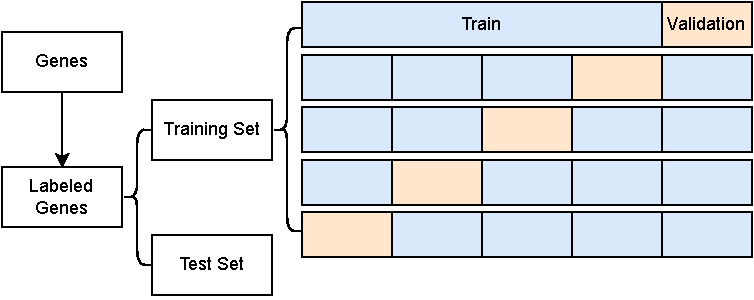
\includegraphics[width=0.9\textwidth]{images/ilustracoes/crossval.pdf}
    \legend{Source: Prepared by the author}
    \label{fig:crossval}
\end{figure*}

Ensuring fairness and reproducibility is crucial for comparing GNN models across different PPI networks. To achieve this, we aimed to maintain a consistent test set throughout the experiments. In the first stage, we accomplished this by setting the \textit{random\_state} parameter of the function used to divide the labeled data into training and test sets. This guarantees that the same test set is employed for each PPI network during the comparative performance evaluation carried out. In the second stage, on the other hand, we aimed to compare not only model predictive performance but also actual predictions for the same set of genes across different PPI networks. Thus, for this stage of our methodology, we manually separated a test set that is common to all PPI networks and used it as a fixed independent test set in the experiments. This process is further discussed in Section \ref{sec:independent_testset}.

For traditional ML algorithms, the performance evaluation was based only on a 5-fold CV process in the complete labeled data. Since in the stage of algorithms comparison, we did not included a step of tuning ML models using hyperparameters optimization, the $k$-fold CV procedure is a reliable approach to conduct model evaluation and extract robust performance estimates.

All models were evaluated based on the Area under the Precision-Recall Curve (AUC-PR), Area under the ROC curve (AUC-ROC), and accuracy. These metrics were defined in Section~\ref{sec:background_modelEvaluation}. Due to the severe class imbalance found in our data and to the negative impact it causes in the model evaluation through accuracy and AUC-ROC, we employed AUC-PR as our main metric.








\section{Construction of ensemble models}
\label{sec:ensemble_training}

Two ensemble models were constructed based on the strategies outlined in Section~\ref{sec:comp_concepts:ensemble}. Our aim was to investigate whether the consensus among a set of predictive models, each of which trained with a specific PPI network as the base graph for learning, can introduce robustness and performance gain to our approach. 

The trained GNN models, regardless of the algorithm used, are able to provide for a given test instance (\ie an unlabeled node referring to an unannotated gene) a predicted class and predicted class probabilities. Since our task is binary classification, we obtain two probabilities for each gene, one for the \textit{Driver} class (positive) and one for the \textit{Passenger} class (negative), with both probabilities summing to one. A higher probability for the positive class indicates a greater likelihood of the gene being a driver gene, according to the model. Thus, two strategies were adopted to obtain ensemble-based predictions:
\begin{itemize}
    \item \textbf{Ensemble-Majority}: combines predicted class labels using majority voting. A gene is classified as a driver if it is predicted as such by at least three PPI networks (\ie models), with ties considered positive due to the even number of networks.
    \item \textbf{Ensemble-Average}: combines class probabilities by taking the average across all six PPI networks (\ie models). A gene is classified as a driver if its average probability for the \textit{Driver} class is equal to or greater than 0.5.
\end{itemize}

Finally, we note that for the purpose of discussing results, we will refer to the GCN trained with UNION PPI network, with the Ensemble-Majority, and with the Ensemble-Average as our ensemble-based prediction models. 








\section{Summary}
This chapter introduced the datasets and the methods explored in this work to build the framework for our comparative analysis among learning algorithms and to develop a graph-based predictive model for identifying CDGs.  The selected pre-processed multi-omics datasets, derived from TCGA, encompass 16 different types of cancer and four levels of omics data, including genomics (SNVs and CNAs), transcriptomics, and epigenomics. Furthermore, six different PPI networks of different dimensions were collected and pre-processed to extract centrality measures and to fit the needs for the application of GNNs. From these networks, a UNION PPI network was generated based on a simple merging of all collected PPI networks. A careful curation of databases was conducted to define the most possible reliable sets of positive and negative examples of CDGs to serve as node labels for model training. Finally, the methodology for model development included strategies for handling class imbalance and for building ensemble models as means to improve the prediction results. The next chapters will detail the application of these materials and methods for a comprehensive experimental investigation of learning algorithms and data representation and for the and the development of a GNN model for CDGs prediction.






